\documentclass[aspectratio=169, 11pt]{beamer}

% ========== 主题设置 ==========
\usetheme{Madrid}
\usecolortheme{whale}
\setbeamertemplate{navigation symbols}{}
\setbeamertemplate{footline}[frame number]

% ========== 包 ==========
\usepackage{tikz}
\usetikzlibrary{arrows.meta, positioning, shapes.geometric, calc, fit, backgrounds}
\usepackage{booktabs}
\usepackage{graphicx}
\usepackage{amsmath}
\usepackage{xcolor}
\usepackage{subcaption}

% ========== 颜色定义 ==========
\definecolor{highlight}{RGB}{255, 100, 100}      % 当前工作模块（红色高亮）
\definecolor{completed}{RGB}{100, 200, 100}      % 已完成模块（绿色）
\definecolor{pending}{RGB}{200, 200, 200}        % 待完成模块（灰色）
\definecolor{inprogress}{RGB}{100, 150, 255}     % 进行中（蓝色）
\definecolor{improved}{RGB}{50, 180, 50}         % 改进（深绿）

% ========== 标题信息 ==========
\title{Weekly Progress Report}
\subtitle{Week 10: BrainFlow Integration \& Movement Amplitude Optimization}
\author{Student ID: 11314389}
\institute{BCI Control System Project}
\date{March 11, 2026}

\begin{document}

% ========== 标题页 ==========
\begin{frame}
    \titlepage
\end{frame}

% ========== Slide 1: 系统架构图 ==========
\begin{frame}{System Overview: Current Focus}
    \begin{center}
    \resizebox{0.95\textwidth}{!}{%
    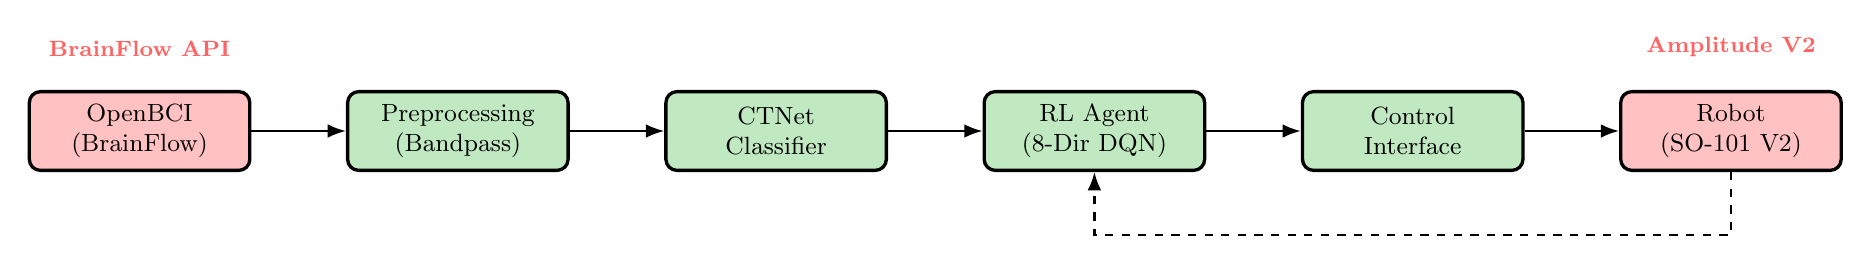
\begin{tikzpicture}[
        node distance=8mm and 12mm,
        block/.style={rectangle, rounded corners, draw, very thick,
                      minimum width=28mm, minimum height=10mm,
                      align=center, font=\small},
        arrow/.style={-Latex, thick},
    ]
        \node[block, fill=highlight!40] (raw) {OpenBCI\\(BrainFlow)};
        \node[block, fill=completed!40, right=of raw] (prep) {Preprocessing\\(Bandpass)};
        \node[block, fill=completed!40, right=of prep] (ctnet) {CTNet\\Classifier};
        \node[block, fill=completed!40, right=of ctnet] (dqn) {RL Agent\\(8-Dir DQN)};
        \node[block, fill=completed!40, right=of dqn] (ctrl) {Control\\Interface};
        \node[block, fill=highlight!40, right=of ctrl] (robot) {Robot\\(SO-101 V2)};
        
        \draw[arrow] (raw) -- (prep);
        \draw[arrow] (prep) -- (ctnet);
        \draw[arrow] (ctnet) -- (dqn);
        \draw[arrow] (dqn) -- (ctrl);
        \draw[arrow] (ctrl) -- (robot);
        
        \draw[arrow, dashed] (robot.south) -- ++(0,-8mm) -| (dqn.south);
        
        \node[above=3mm of raw, highlight, font=\footnotesize\bfseries] {BrainFlow API};
        \node[above=3mm of robot, highlight, font=\footnotesize\bfseries] {Amplitude V2};
        
    \end{tikzpicture}}
    \end{center}
    
    \vspace{3mm}
    \begin{columns}[T]
        \column{0.5\textwidth}
        \textbf{Legend:}
        \begin{itemize}
            \item[\textcolor{completed}{\rule{8pt}{8pt}}] Completed
            \item[\textcolor{inprogress}{\rule{8pt}{8pt}}] In Progress
        \end{itemize}
        \column{0.5\textwidth}
        \begin{itemize}
            \item[\textcolor{highlight}{\rule{8pt}{8pt}}] \textbf{This Week's Focus}
            \item[\textcolor{pending}{\rule{8pt}{8pt}}] Pending
        \end{itemize}
    \end{columns}
\end{frame}

% ========== Slide 2: 本周目标 ==========
\begin{frame}{This Week's Objectives}
    \begin{block}{Goals}
        \begin{enumerate}
            \item Integrate BrainFlow API for real-time EEG data acquisition (OpenBCI)
            \item Optimize robot arm movement amplitude for clearer visual observation
            \item Fix arm trembling at hardware limits (boundary clamping)
            \item Compare V1 vs V2 control accuracy with proper error unit definition
        \end{enumerate}
    \end{block}
    
    \vspace{5mm}
    
    \begin{alertblock}{Key Question to Address}
        Can increased movement amplitude reduce relative positioning error, and does BrainFlow real-time EEG integration maintain the same control quality?
    \end{alertblock}
\end{frame}

% ========== Slide 3: 方法/实现 ==========
\begin{frame}{Methods \& Implementation}
    \begin{columns}[T]
        \column{0.5\textwidth}
        \textbf{V2 Amplitude Optimization:}
        \begin{itemize}
            \item Decreased \texttt{norm\_step}: $0.25 \to 0.10$
            \item Increased \texttt{max\_steps}: $30 \to 50$
            \item Physical amplitude $\approx 2.5\times$ larger
            \item Removed software limits (\texttt{margin=0})
            \item Hardware limit clamping added
        \end{itemize}
        
        \vspace{2mm}
        \textbf{Hardware Clamping:}
        \begin{equation*}
            \text{target} = \text{clamp}(\text{cur} + \Delta, \text{min}_{\text{hw}}, \text{max}_{\text{hw}})
        \end{equation*}
        
        \column{0.5\textwidth}
        \textbf{BrainFlow Integration:}
        \begin{itemize}
            \item \texttt{SYNTHETIC\_BOARD} (default)
            \item \texttt{CYTON\_BOARD} (physical OpenBCI)
            \item Real-time 8--30 Hz bandpass filter
            \item CTNet 4-class MI classification
            \item 1-second epoch per control step
        \end{itemize}
        
        \vspace{2mm}
        \textbf{New Scripts:}
        \begin{itemize}
            \item \texttt{test\_8dir\_comprehensive\_v2.py}
            \item \texttt{brainflow\_physical\_control.py}
        \end{itemize}
    \end{columns}
\end{frame}

% ========== Slide 4: Error Unit Definition ==========
\begin{frame}{Unified Error Metric Definition}
    \begin{block}{Metric: Endpoint Error (Final Distance to Target)}
    \small
    All errors measure the \textbf{Euclidean distance} from final position to target in \textbf{normalized coordinates} $[-1, 1]$. \\
    Workspace\% $= \frac{\text{error}}{2.0} \times 100\%$ provides a version-independent comparison. Reach threshold: $d < 0.12$ ($6\%$).
    \end{block}
    
    \vspace{1mm}
    
    \begin{columns}[T]
        \column{0.5\textwidth}
        \textbf{V1 vs V2 Parameter Differences:}
        \begin{table}
            \centering
            \footnotesize
            \begin{tabular}{lcc}
                \toprule
                Parameter & V1 & V2 \\
                \midrule
                \texttt{step\_rad} & 0.35 & 0.70 \\
                \texttt{norm\_step} & 0.12 & 0.10 \\
                rad/norm & 2.92 & 7.00 \\
                $1 \text{ step} \to$ & $20.1^\circ$ & $40.1^\circ$ \\
                \bottomrule
            \end{tabular}
        \end{table}
        
        \column{0.5\textwidth}
        \textbf{Why Workspace\% is Preferred:}
        \begin{itemize}
            \item Independent of \texttt{step\_rad}/\texttt{norm\_step}
            \item Directly comparable across V1/V2
            \item Intuitive: ``error as fraction of total range''
        \end{itemize}
        
        \vspace{1mm}
        \textbf{Formula:} $d = \sqrt{(\Delta y)^2 + (\Delta z)^2}$
    \end{columns}
\end{frame}

% ========== Slide 5: V2 Test - Horizontal & Vertical ==========
\begin{frame}{V2 Physical Test: Horizontal \& Vertical Movement}
    \begin{columns}[T]
        \column{0.5\textwidth}
        \textbf{Horizontal Movement:}
        \begin{center}
            
\includegraphics[width=0.92\textwidth]{../outputs/8dir_comprehensive_test_v2/a_horizontal.png}
        \end{center}
        
        \column{0.5\textwidth}
        \textbf{Vertical Movement:}
        \begin{center}
            
\includegraphics[width=0.92\textwidth]{../outputs/8dir_comprehensive_test_v2/b_vertical.png}
        \end{center}
    \end{columns}
    
    \vspace{2mm}
    \textbf{Observations:}
    \begin{itemize}
        \item Increased amplitude makes movements clearly visible on the robot
        \item Mean error: 0.100 normalized (5.0\% of workspace, $0.70$ rad / $40.1^\circ$)
    \end{itemize}
\end{frame}

% ========== Slide 6: V2 Test - Diagonal ==========
\begin{frame}{V2 Physical Test: Diagonal Movement}
    \begin{columns}[T]
        \column{0.5\textwidth}
        \textbf{Diagonal UL-DR:}
        \begin{center}
            
\includegraphics[width=0.92\textwidth]{../outputs/8dir_comprehensive_test_v2/c_diagonal_ul_dr.png}
        \end{center}
        
        \column{0.5\textwidth}
        \textbf{Diagonal UR-DL:}
        \begin{center}
            
\includegraphics[width=0.92\textwidth]{../outputs/8dir_comprehensive_test_v2/d_diagonal_ur_dl.png}
        \end{center}
    \end{columns}
    
    \vspace{2mm}
    \textbf{Observations:}
    \begin{itemize}
        \item Simultaneous Y/Z movement confirms true 8-direction capability
        \item Mean error: 0.101 normalized (5.1\%, $0.71$ rad / $40.5^\circ$)
    \end{itemize}
\end{frame}

% ========== Slide 7: V2 Test - Square ==========
\begin{frame}{V2 Physical Test: Square Movement Patterns}
    \begin{columns}[T]
        \column{0.5\textwidth}
        \textbf{Square Clockwise:}
        \begin{center}
            
\includegraphics[width=0.92\textwidth]{../outputs/8dir_comprehensive_test_v2/e_square_cw.png}
        \end{center}
        
        \column{0.5\textwidth}
        \textbf{Square Counter-Clockwise:}
        \begin{center}
            
\includegraphics[width=0.92\textwidth]{../outputs/8dir_comprehensive_test_v2/f_square_ccw.png}
        \end{center}
    \end{columns}
    
    \vspace{2mm}
    \textbf{Observations:}
    \begin{itemize}
        \item All 12 targets per pattern reached (100\% reach rate)
        \item Mean error: 0.062 normalized (3.1\%, $0.43$ rad / $24.9^\circ$) --- best among all patterns
    \end{itemize}
\end{frame}

% ========== Slide 8: V2 All Patterns Overview ==========
\begin{frame}{V2 Physical Test: All Patterns Overview}
    \begin{center}
        
\includegraphics[width=0.82\textwidth,height=0.65\textheight,keepaspectratio]{../outputs/8dir_comprehensive_test_v2/all_pos_vs_time.png}
    \end{center}
    
    \textbf{Summary:} All 48/48 targets reached (100\%). Larger amplitude enables clear observation of each movement pattern on the physical robot arm.
\end{frame}

% ========== Slide 9: BrainFlow Integration Results ==========
\begin{frame}{BrainFlow Pipeline Integration (Guided Mode)}
    \begin{center}
        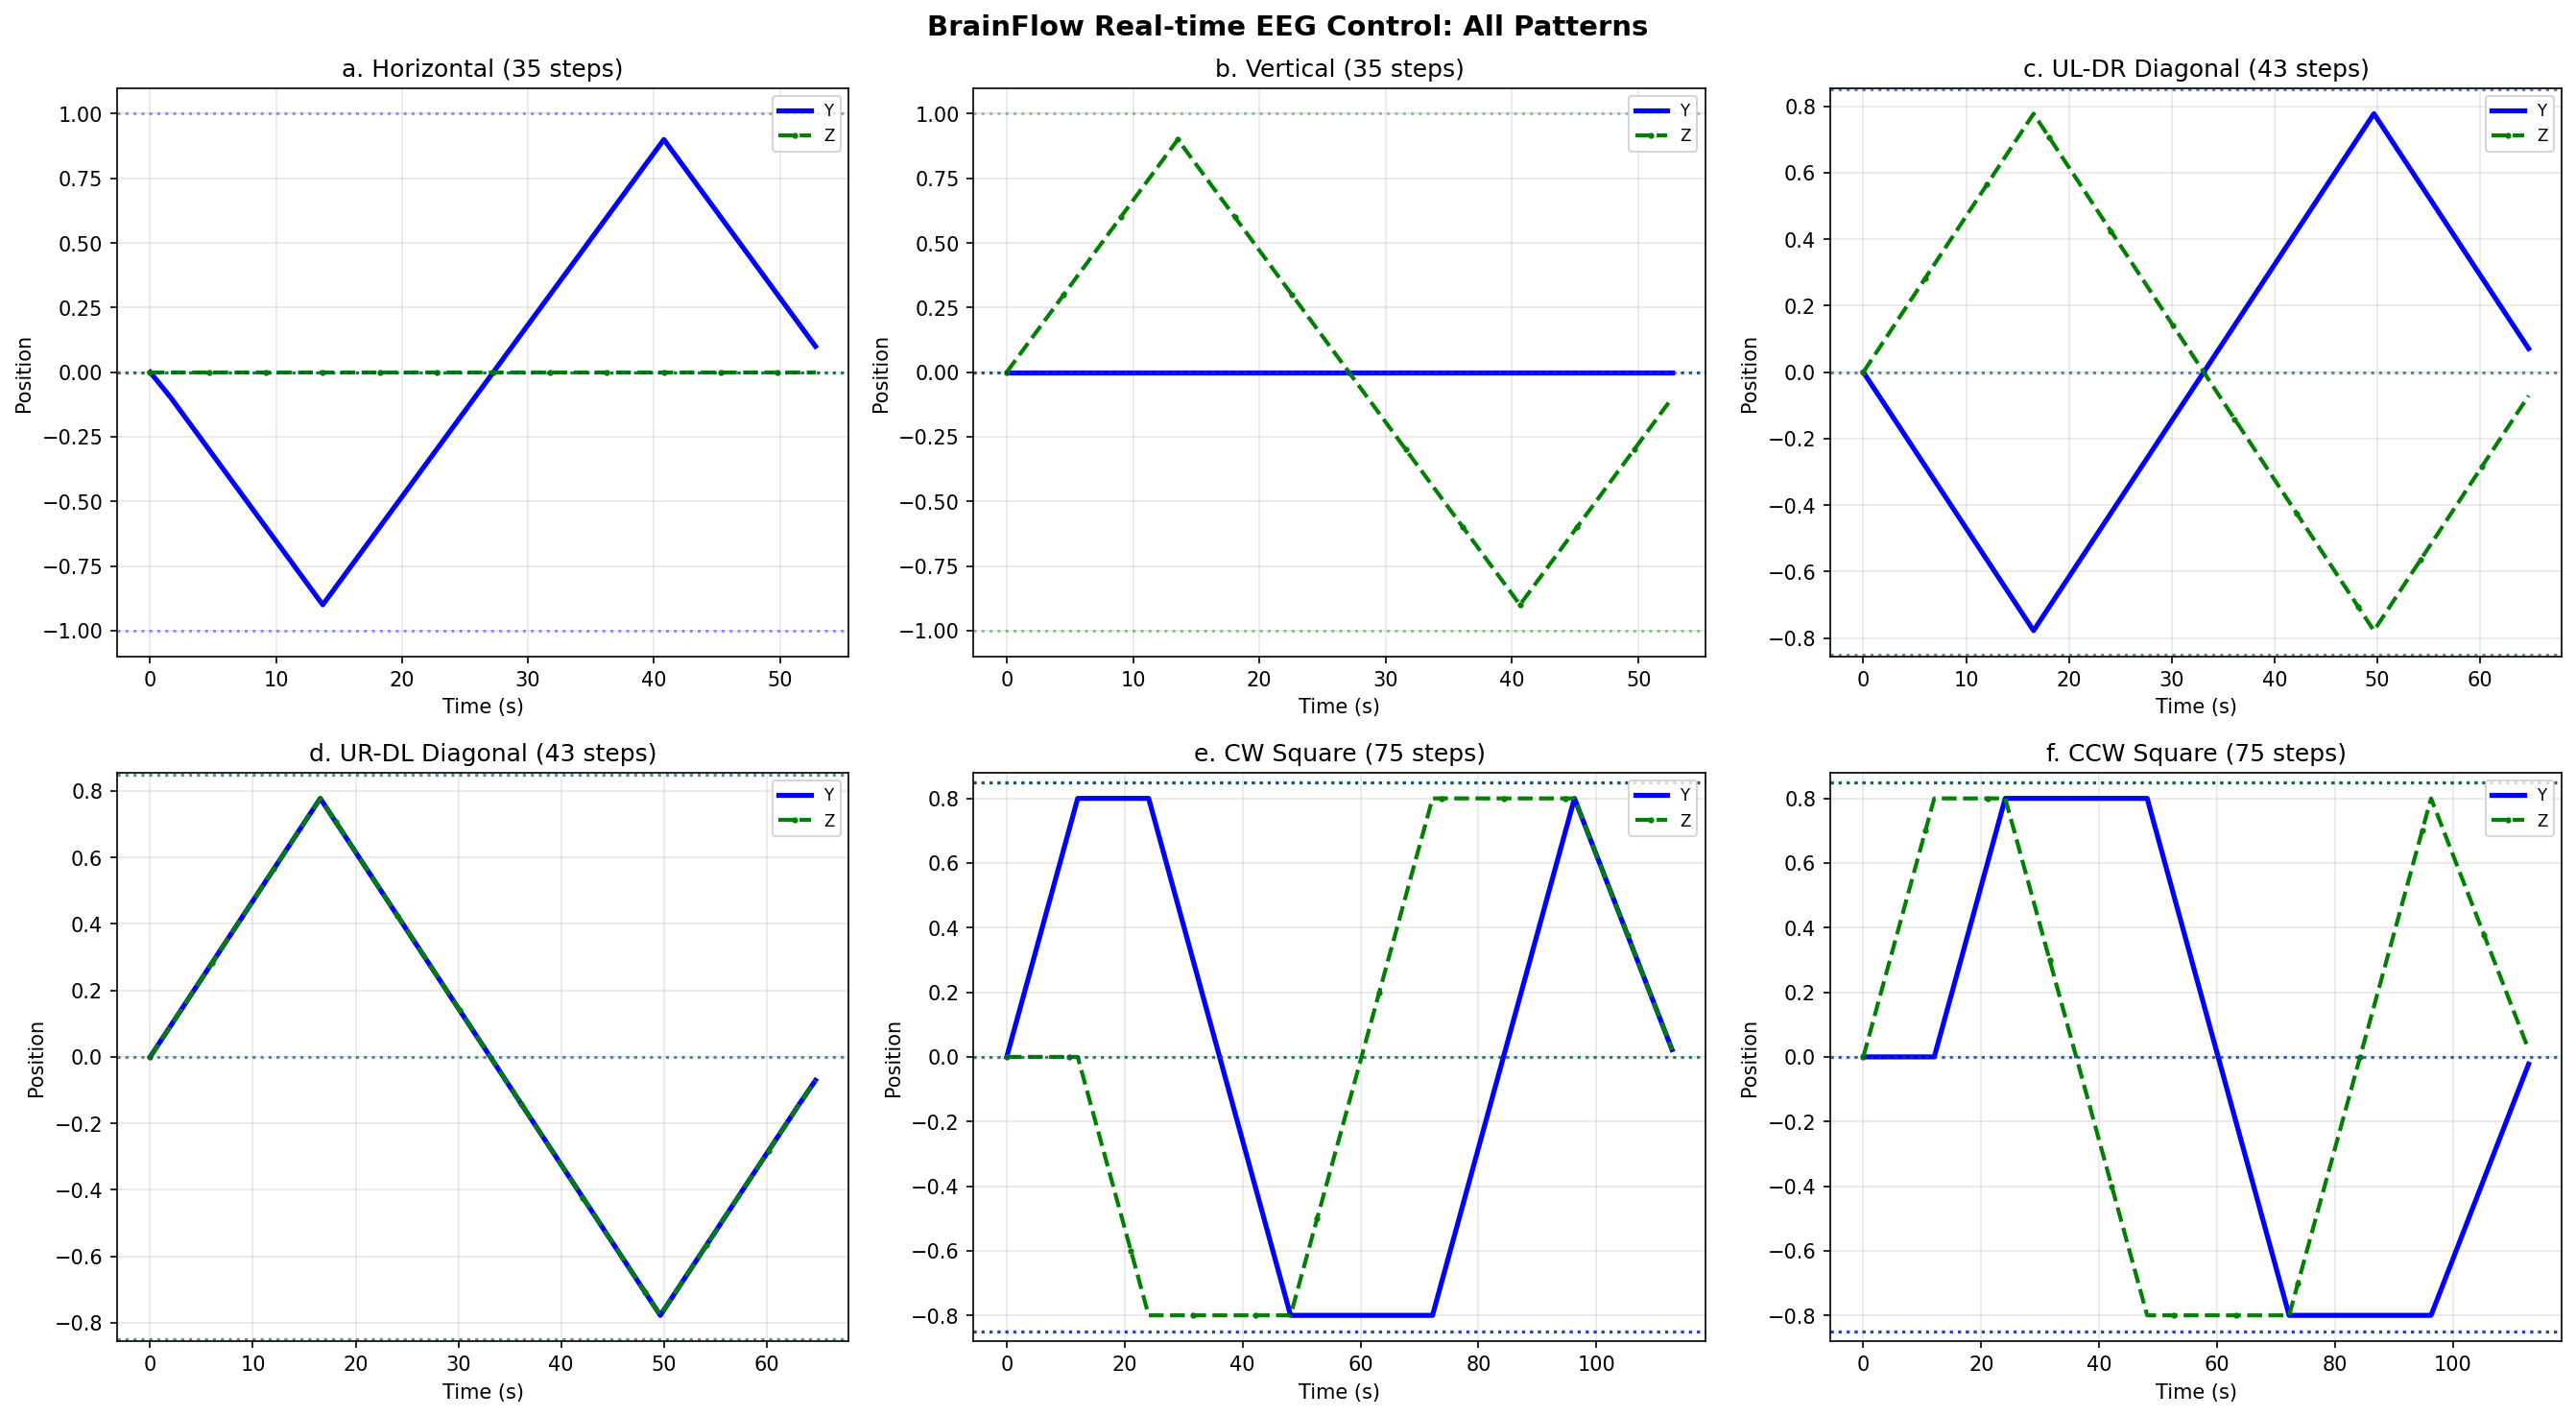
\includegraphics[width=0.82\textwidth,height=0.58\textheight,keepaspectratio]{../outputs/brainflow_physical_control/all_pos_vs_time.png}
    \end{center}
    
    \vspace{1mm}
    \textbf{Pipeline:} OpenBCI (Synthetic) $\to$ BrainFlow $\to$ Bandpass $\to$ CTNet $\to$ \textit{(logged only)} \\
    \textbf{Control:} Guided mode --- correct action used, EEG classified but \textbf{not used for control}. \\
    \textbf{Purpose:} Validates engineering pipeline stability, not BCI classification quality.
\end{frame}

% ========== Slide 10: BrainFlow EEG Classification ==========
\begin{frame}{BrainFlow: EEG Classification Analysis}
    \begin{center}
        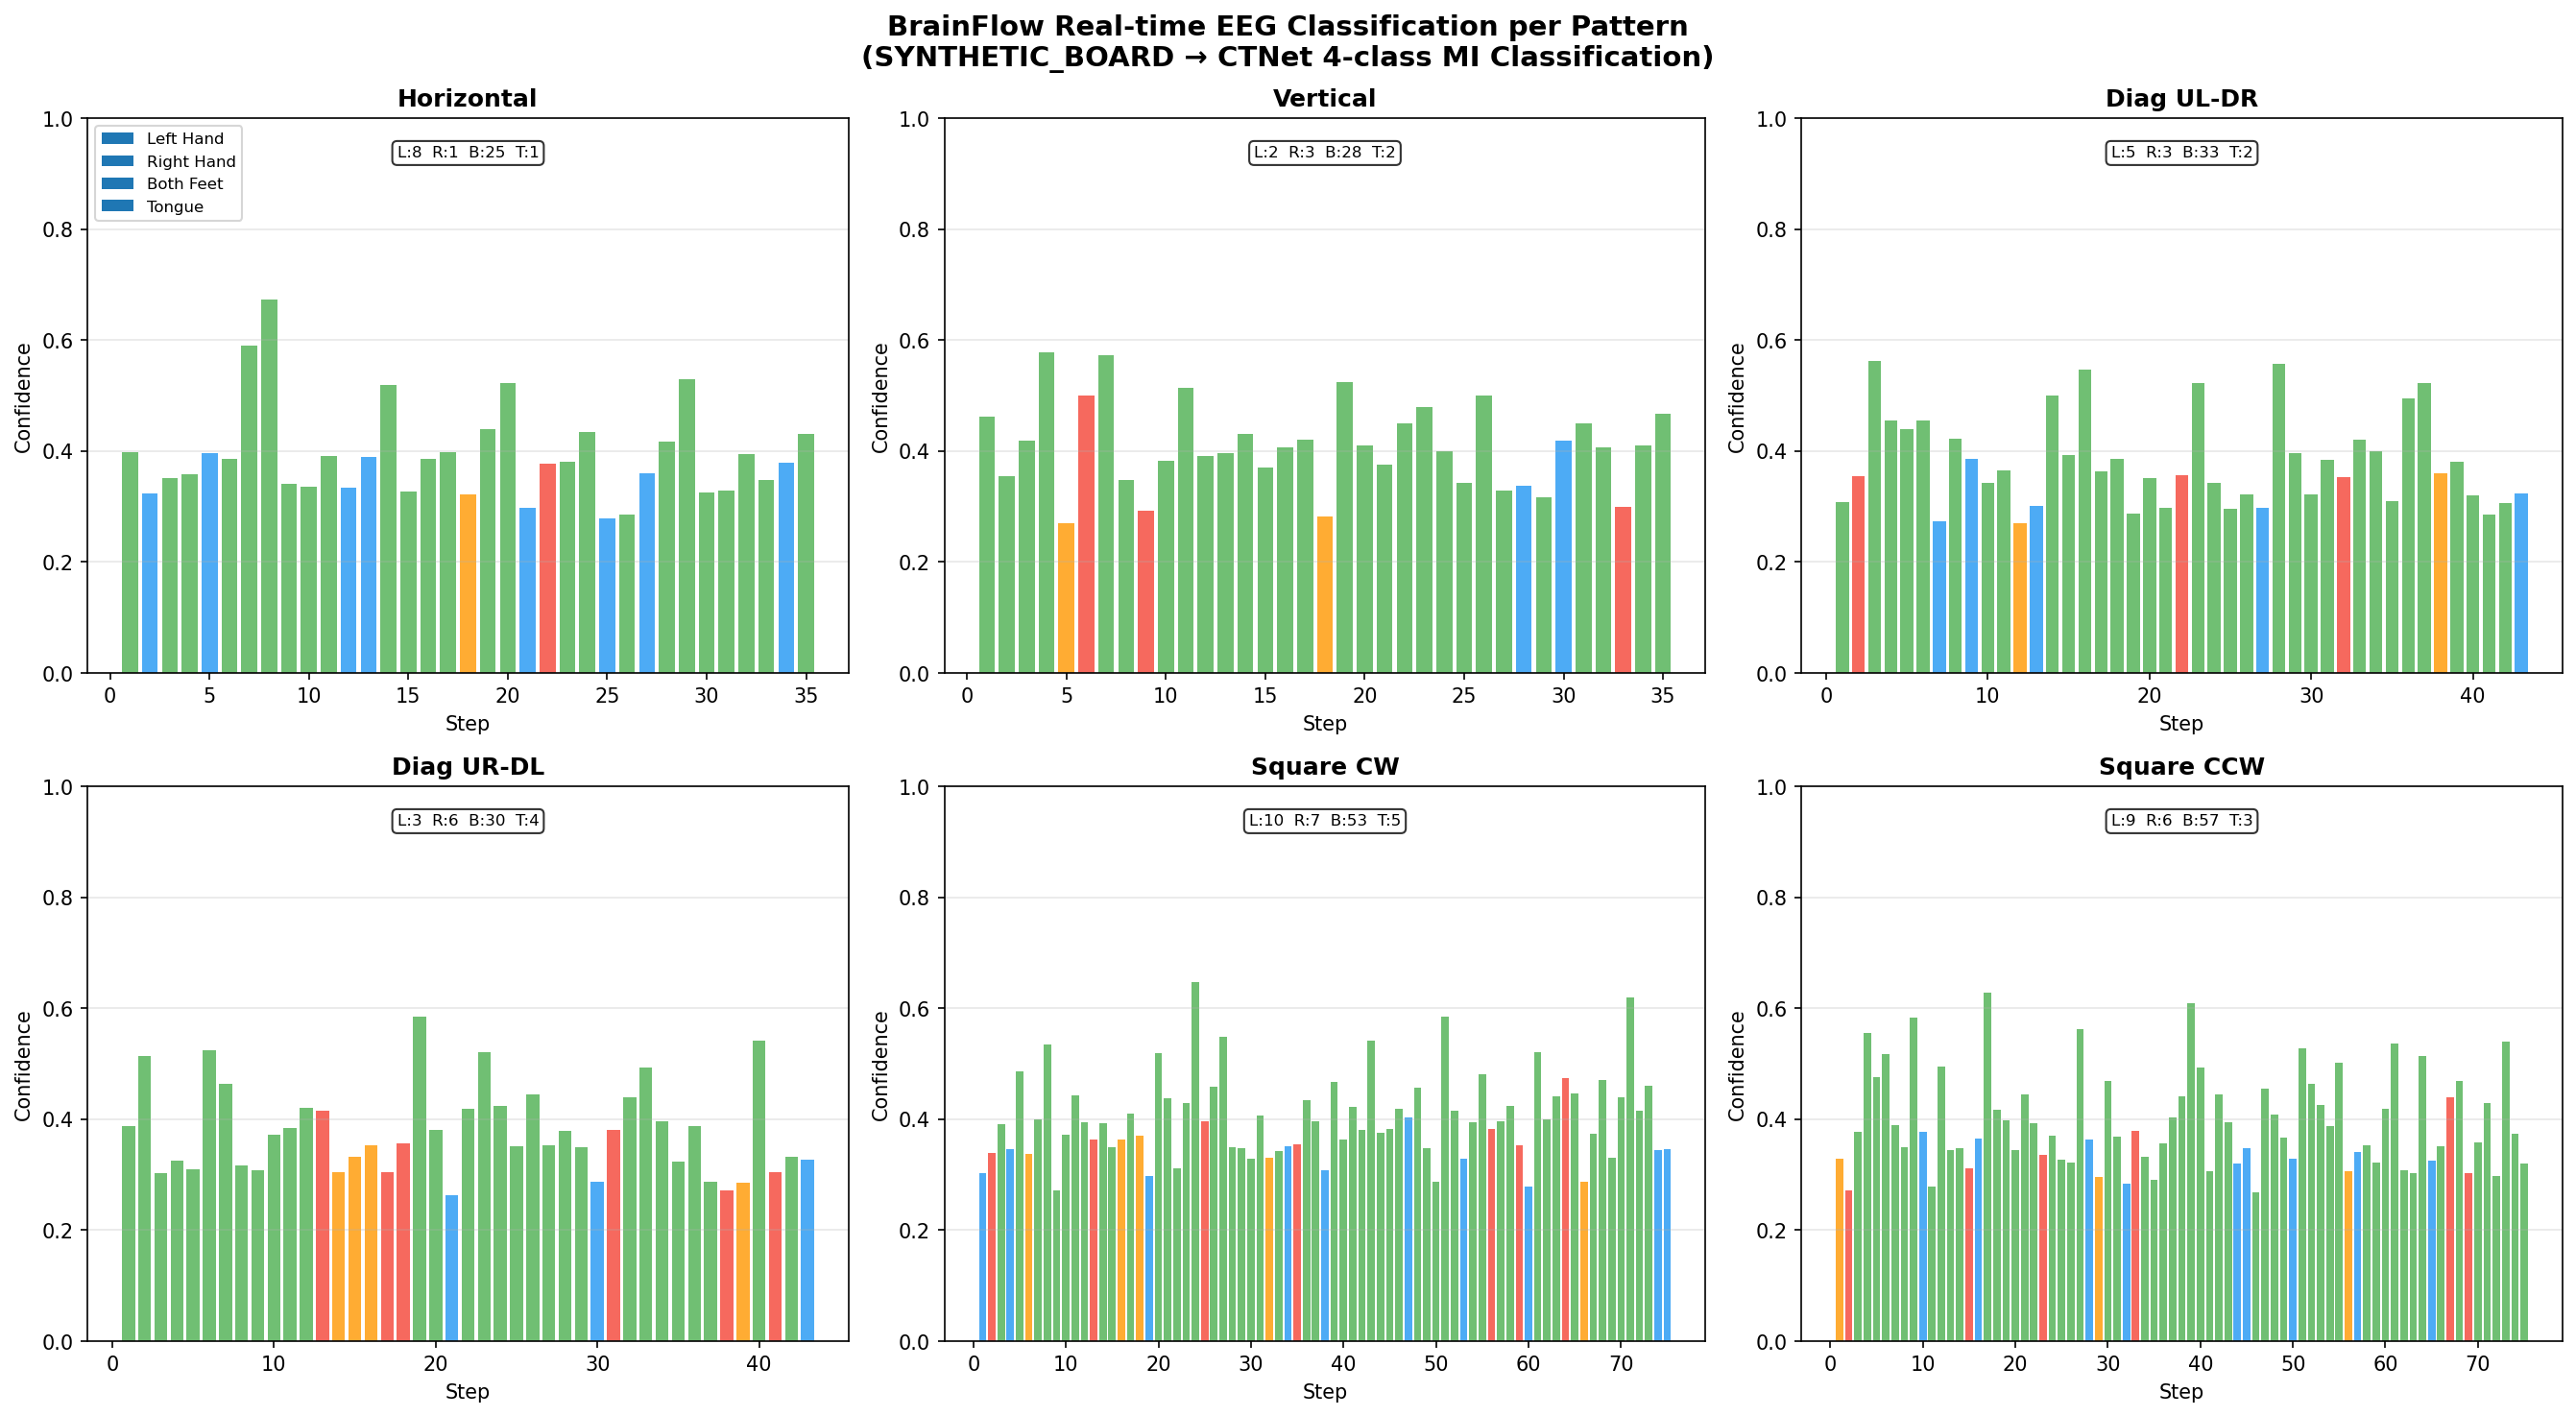
\includegraphics[width=0.85\textwidth,height=0.60\textheight,keepaspectratio]{../outputs/comparison_v1_v2_brainflow/brainflow_eeg_classification.png}
    \end{center}
    
    \vspace{1mm}
    \textbf{Analysis:} CTNet classifies real-time synthetic EEG into 4 MI classes. Guided mode uses the correct action but still reads and classifies EEG each step.
\end{frame}

% ========== Slide 11: Unified Comparison ==========
\begin{frame}{Unified Endpoint Error Comparison (All Datasets)}
    \begin{center}
        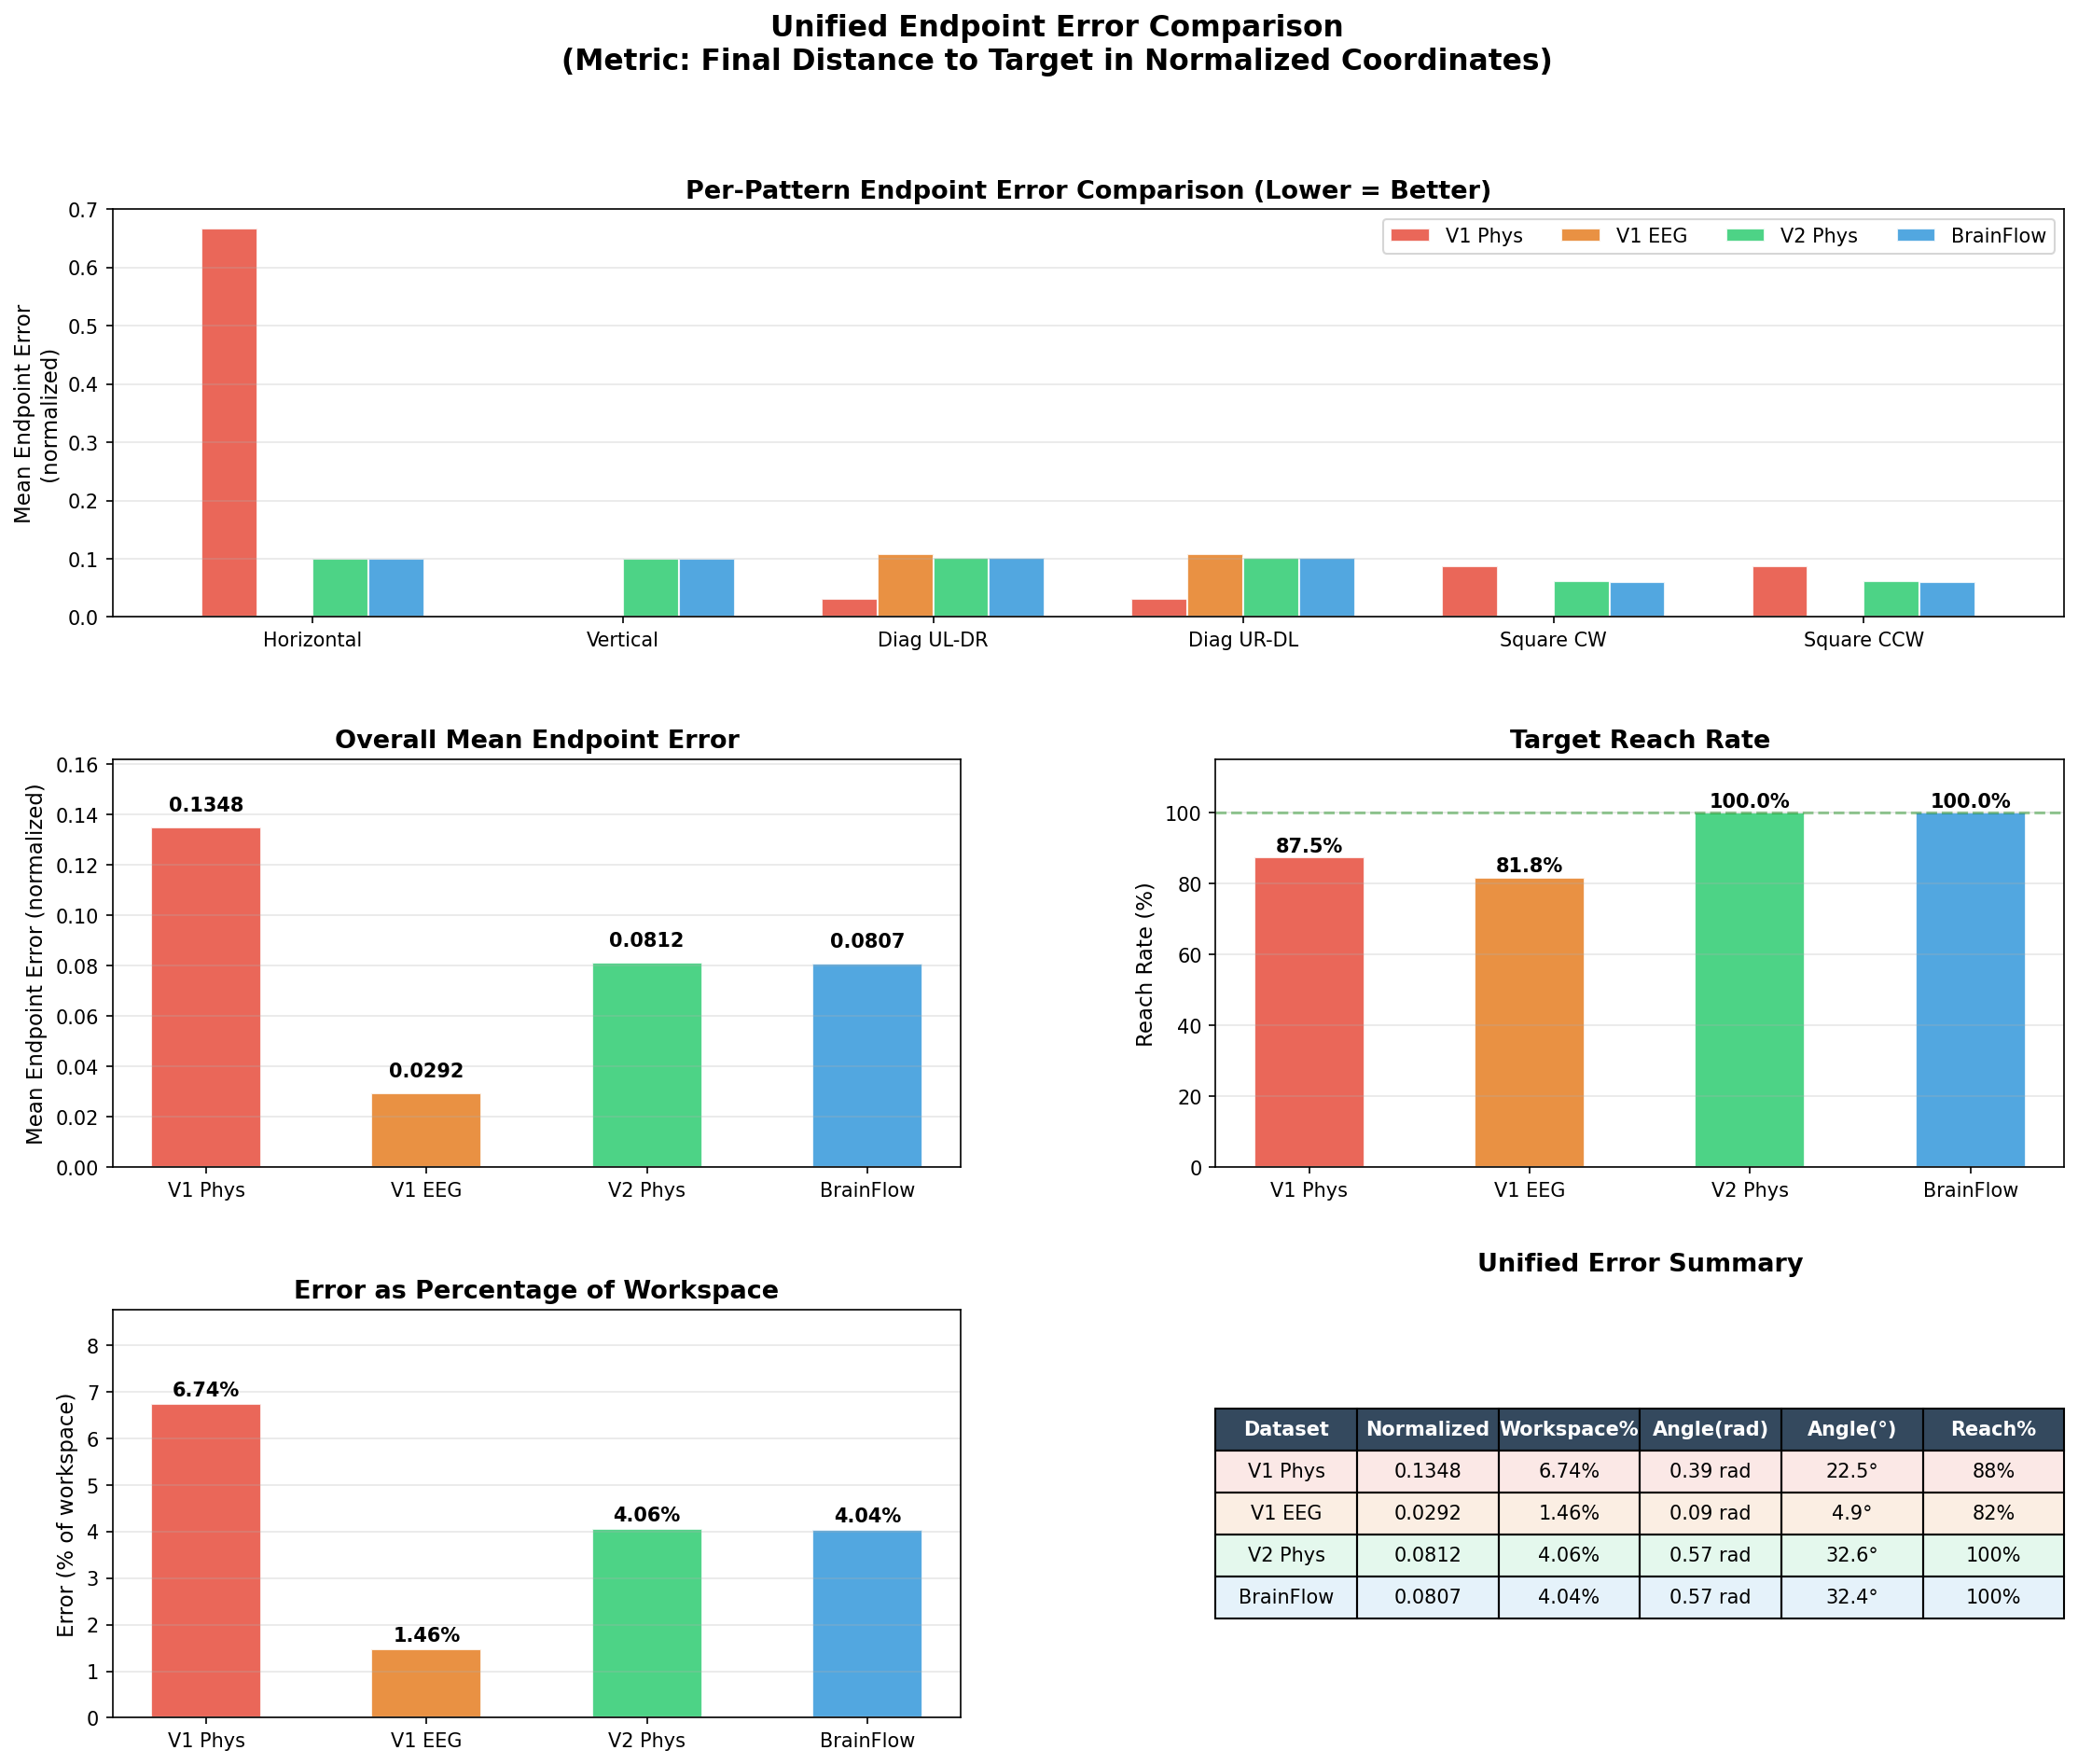
\includegraphics[width=0.92\textwidth,height=0.65\textheight,keepaspectratio]{../outputs/comparison_v1_v2_brainflow/unified_error_comparison.png}
    \end{center}
    
    \vspace{1mm}
    \footnotesize
    \textbf{Note:} All current tests use \textbf{guided/ideal actions} (not EEG-driven). ``V1 EEG'' adds 10\% random noise to simulate classification error. Next step: real MI-driven control using PhysioNet-trained CTNet.
\end{frame}

% ========== Slide 12: BrainFlow Pipeline Validation ==========
\begin{frame}{BrainFlow Pipeline Validation (Guided Mode)}
    \begin{columns}[T]
        \column{0.55\textwidth}
        \begin{center}
            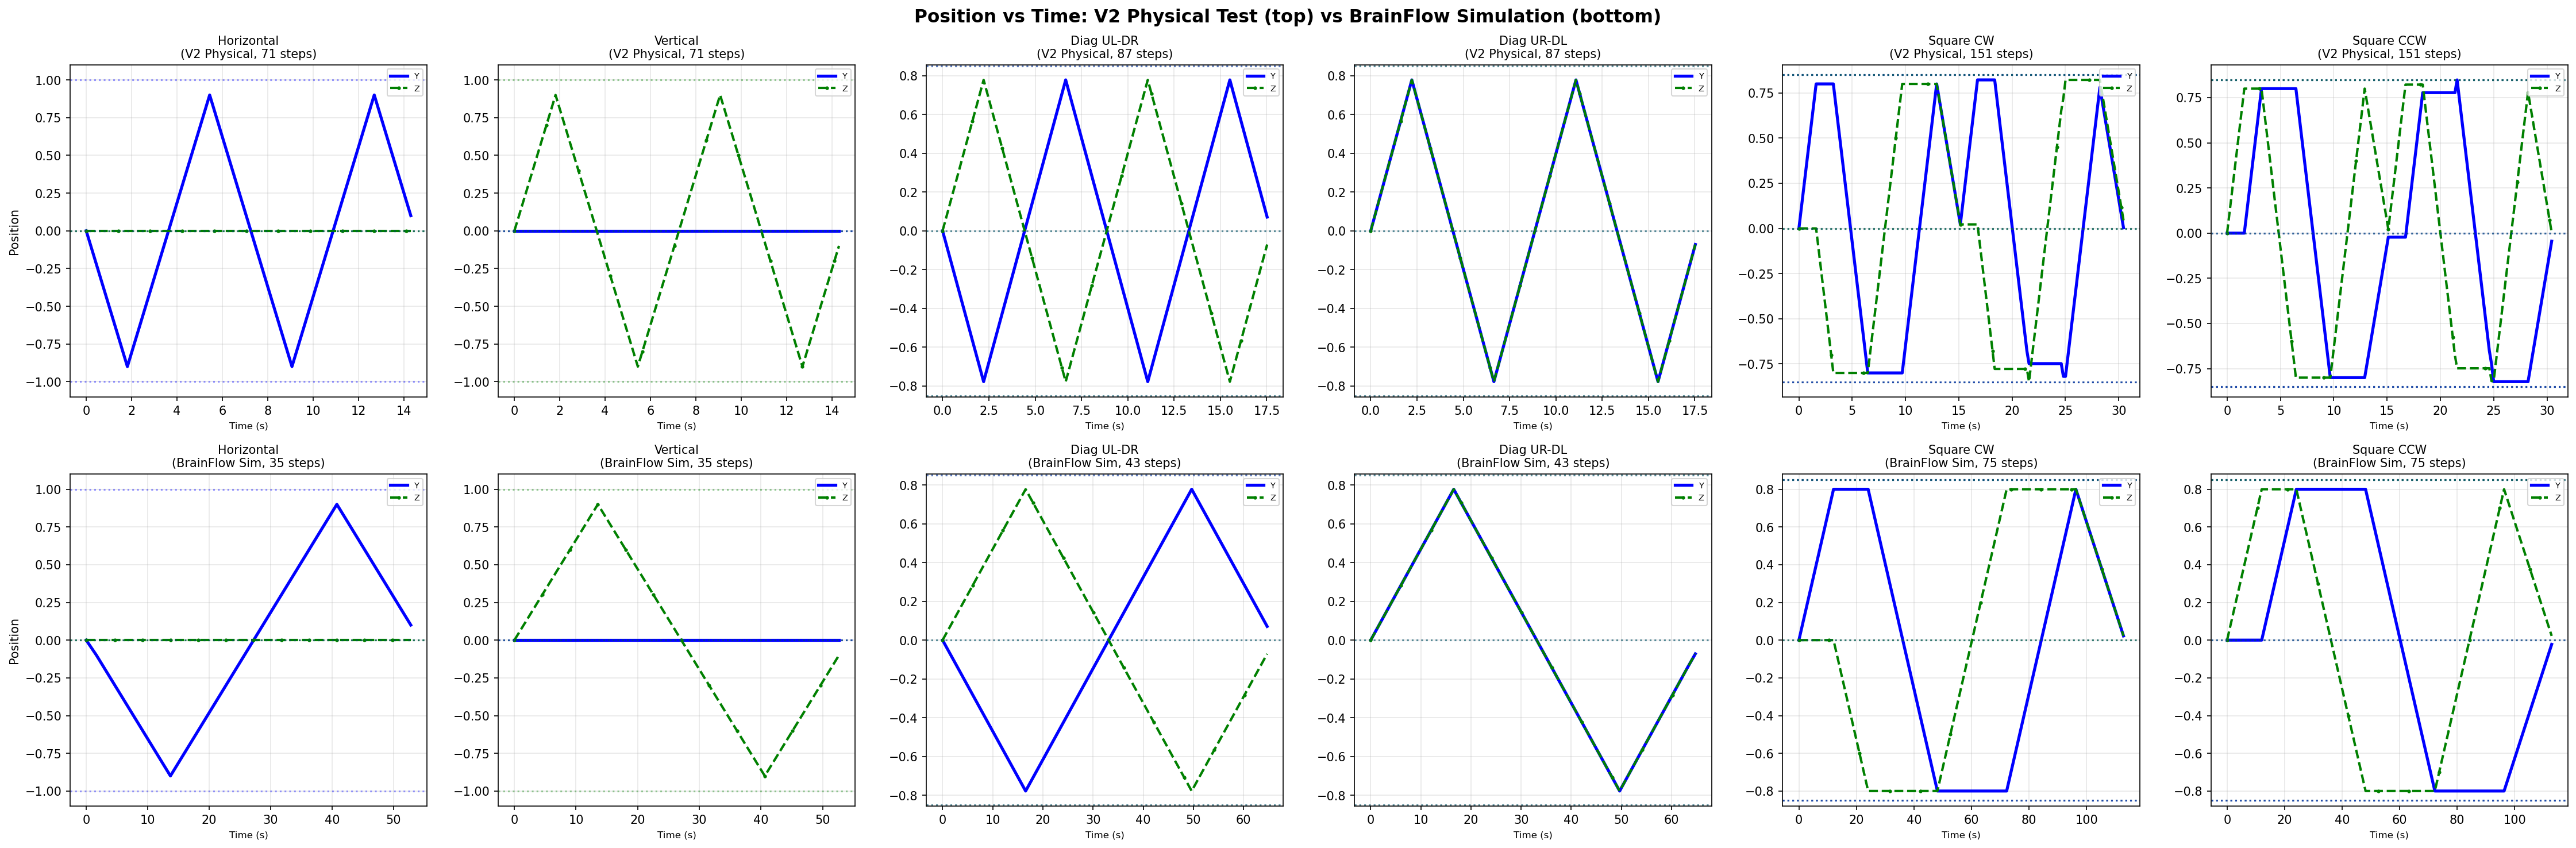
\includegraphics[width=\textwidth,height=0.55\textheight,keepaspectratio]{../outputs/comparison_v1_v2_brainflow/v2_vs_brainflow_pos_vs_time.png}
        \end{center}
        
        \column{0.45\textwidth}
        \textbf{What guided mode validates:}
        \begin{itemize}
            \item BrainFlow data acquisition stable
            \item Real-time bandpass filtering works
            \item CTNet inference runs every 1s epoch
            \item Control loop runs without crash
        \end{itemize}
        
        \vspace{2mm}
        \begin{alertblock}{Limitation}
            \footnotesize
            Guided mode uses \textbf{correct action}, not CTNet prediction. Trajectories match V2 by design --- this proves \textbf{engineering readiness}, not BCI control quality.
        \end{alertblock}
    \end{columns}
    
    \vspace{2mm}
    \textbf{Next step:} Free mode with real MI data (OpenBCI Cyton or replayed BCI-IV signals) to validate actual EEG-driven control.
\end{frame}

% ========== Slide 13: Challenges & Solutions ==========
\begin{frame}{Challenges \& Solutions}
    \begin{columns}[T]
        \column{0.5\textwidth}
        \begin{alertblock}{Challenges Encountered}
            \begin{itemize}
                \item Arm trembles when moving left (hardware limit hit)
                \item V1 position tracking always reads (0,0) due to bug
                \item \texttt{brainflow} not installed in Conda env
                \item Movement amplitude too small for visual observation
            \end{itemize}
        \end{alertblock}
        
        \column{0.5\textwidth}
        \begin{exampleblock}{Solutions Applied}
            \begin{itemize}
                \item \texttt{\_clamp\_to\_hw\_limits()} prevents servo oscillation at boundaries
                \item Fixed \texttt{\_y}/\texttt{\_z} update in \texttt{execute\_action()}
                \item Installed \texttt{brainflow} in BCIRL Conda environment
                \item Reduced \texttt{norm\_step} + increased \texttt{max\_steps} for $2.5\times$ amplitude
            \end{itemize}
        \end{exampleblock}
    \end{columns}
    
    \vspace{3mm}
    \textbf{Hardware Limit Clamping (Key Fix):}
    \begin{equation*}
        \text{target}_{\text{safe}} = \max\!\big(\text{min}_{\text{hw}},\ \min(\text{max}_{\text{hw}},\ \text{cur} + \Delta_{\text{ticks}})\big)
    \end{equation*}
\end{frame}

% ========== Slide 14: Results Summary ==========
\begin{frame}{Results Summary (Unified Endpoint Error)}
    \begin{columns}[T]
        \column{0.55\textwidth}
        \textbf{Cross-Version Comparison:}
        \begin{table}
            \centering
            \small
            \begin{tabular}{lccc}
                \toprule
                Dataset & Error & WS\% & Reach \\
                \midrule
                V1 Ideal & 0.135 & 6.74\% & 87.5\% \\
                V1 +10\% noise & 0.036 & 1.79\% & 81.8\% \\
                V2 Ideal & 0.081 & 4.06\% & \textcolor{improved}{\textbf{100\%}} \\
                BF Guided & 0.081 & 4.04\% & \textcolor{improved}{\textbf{100\%}} \\
                \bottomrule
            \end{tabular}
        \end{table}
        \footnotesize \textit{All use ideal/guided actions, not EEG-driven.}
        
        \column{0.45\textwidth}
        \textbf{Pipeline Status:}
        \begin{table}
            \centering
            \small
            \begin{tabular}{lc}
                \toprule
                Component & Status \\
                \midrule
                BrainFlow API & \textcolor{improved}{Ready} \\
                CTNet Inference & \textcolor{improved}{Ready} \\
                Arm Control V2 & \textcolor{improved}{Ready} \\
                MI-driven ctrl & \textcolor{highlight}{Next} \\
                \bottomrule
            \end{tabular}
        \end{table}
    \end{columns}
    
    \vspace{3mm}
    \begin{block}{Key Achievement}
        All engineering components validated independently. Unified error metric established. \textbf{Next step:} train CTNet on PhysioNet MI data and use real classification to drive the robot arm (free mode).
    \end{block}
\end{frame}

% ========== Slide 15: 下周计划 ==========
\begin{frame}{Next Week's Plan}
    \begin{block}{Planned Tasks}
        \begin{enumerate}
            \item Train CTNet on PhysioNet EEGMMIDB (109 subjects, 64ch, 4-class MI)
            \item Implement \textbf{free mode}: CTNet classification drives robot arm directly
            \item Compare guided mode (100\% reach) vs free mode (EEG-driven) trajectories
            \item Quantify impact of classification accuracy on control performance
        \end{enumerate}
    \end{block}
    
    \vspace{3mm}
    
    \begin{columns}[T]
        \column{0.5\textwidth}
        \textbf{Expected Deliverables:}
        \begin{itemize}
            \item PhysioNet-trained CTNet model
            \item Free mode: MI-driven arm control
            \item Guided vs Free error comparison
            \item Classification accuracy vs reach rate
        \end{itemize}
        
        \column{0.5\textwidth}
        \textbf{Key Question:}
        \begin{alertblock}{}
            \footnotesize
            At what classification accuracy does the robot arm achieve acceptable control? How does real MI classification error affect trajectory quality compared to simulated noise?
        \end{alertblock}
    \end{columns}
\end{frame}

% ========== Slide 16: 时间线 ==========
\begin{frame}{Project Timeline}
    \begin{center}
    \resizebox{0.9\textwidth}{!}{%
    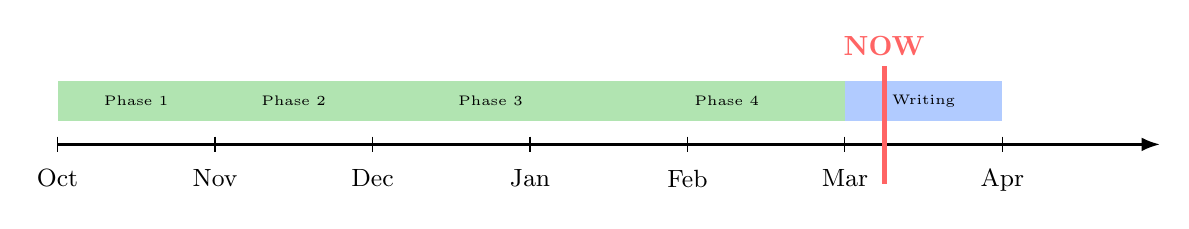
\begin{tikzpicture}
        % 时间轴
        \draw[thick, -Latex] (0,0) -- (14,0);
        
        % 月份标记
        \foreach \x/\month in {0/Oct, 2/Nov, 4/Dec, 6/Jan, 8/Feb, 10/Mar, 12/Apr} {
            \draw (\x, 0.1) -- (\x, -0.1);
            \node[below] at (\x, -0.2) {\small \month};
        }
        
        % 阶段块
        \fill[completed!50] (0, 0.3) rectangle (2, 0.8);
        \node at (1, 0.55) {\tiny Phase 1};
        
        \fill[completed!50] (2, 0.3) rectangle (4, 0.8);
        \node at (3, 0.55) {\tiny Phase 2};
        
        \fill[completed!50] (4, 0.3) rectangle (7, 0.8);
        \node at (5.5, 0.55) {\tiny Phase 3};
        
        \fill[completed!50] (7, 0.3) rectangle (10, 0.8);
        \node at (8.5, 0.55) {\tiny Phase 4};
        
        \fill[inprogress!50] (10, 0.3) rectangle (12, 0.8);
        \node at (11, 0.55) {\tiny Writing};
        
        % 当前位置
        \draw[highlight, ultra thick] (10.5, -0.5) -- (10.5, 1);
        \node[highlight, above] at (10.5, 1) {\textbf{NOW}};
        
    \end{tikzpicture}}
    \end{center}
    
    \vspace{3mm}
    \textbf{Current Status:} On track --- Technical integration complete, entering final documentation \& report writing phase
\end{frame}

\end{document}
